\chapter{N-Gram Graph}

While doing the analysis of the n-gram distribution in Chapter~\ref{}, we started thinking about how we could visualize the structure and distribution of n-grams. We came up with the idea of building a graph, where an edge is present if either the last word of an n-gram matches the first word of another n-gram or the other way around. We even started writing scripts to visualize them, but in the end, we did not find a appropriate place for them in the thesis. Nevertheless, we still include them here to show what it would have looked like.

\begin{figure}[H]
	\minipage{1\textwidth}
	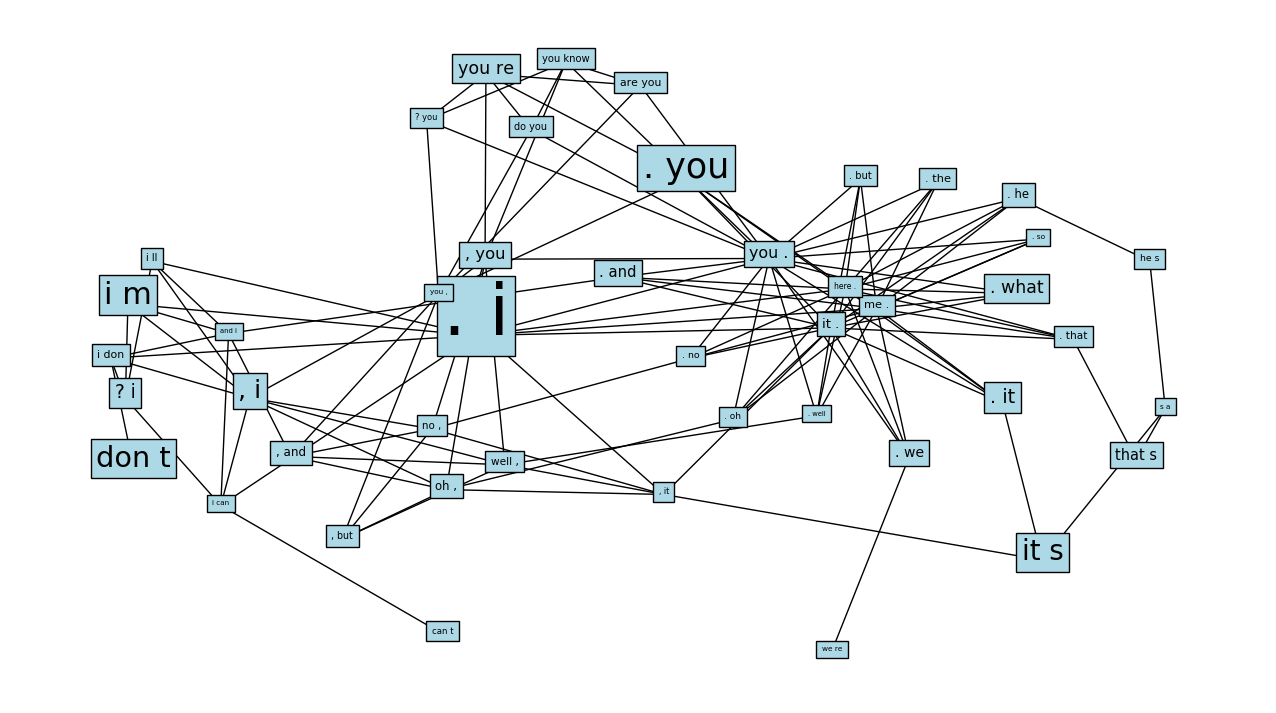
\includegraphics[width=\linewidth]{img/opensubtitles_bigram_top_50_graph}
	\centering
	\small
	\text{OpenSubtitles}
	\endminipage\hfill
	\minipage{1\textwidth}
	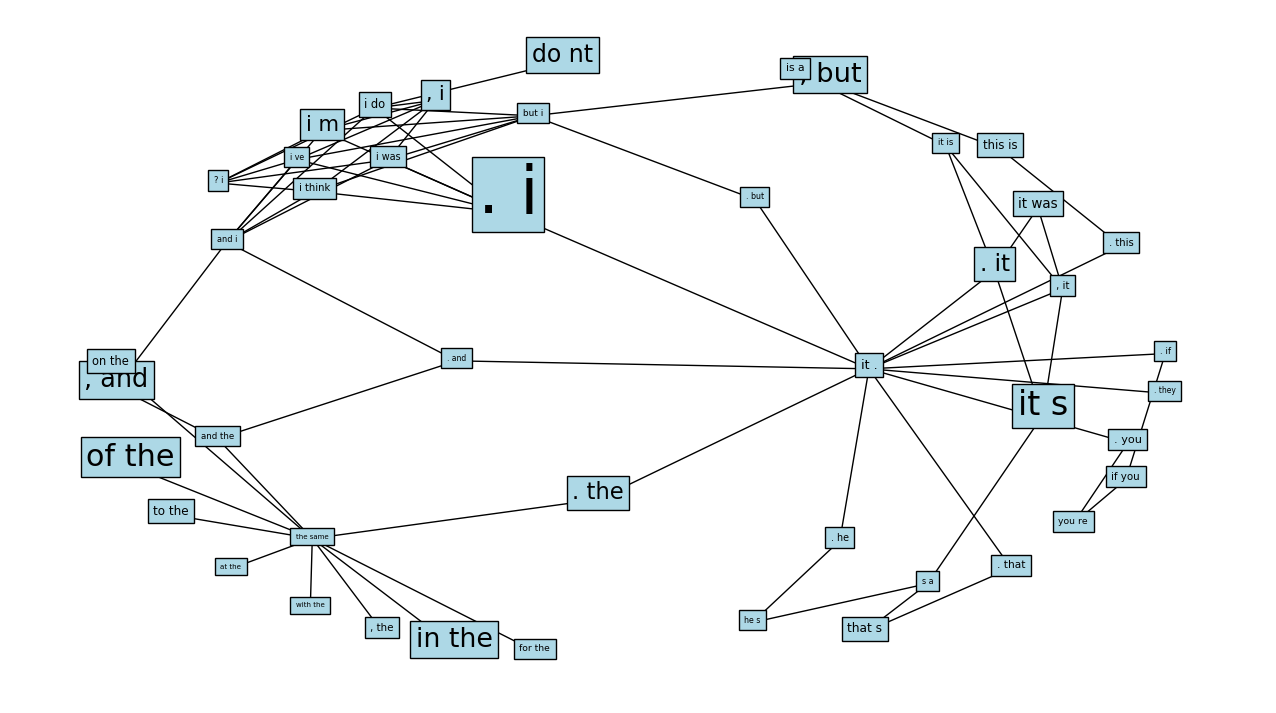
\includegraphics[width=\linewidth]{img/reddit_bigram_top_50_graph}
	\centering
	\small
	\text{Reddit}
	\endminipage\hfill
	\caption{N-Gram graphs for the 50 most used bigrams in the OpenSubtitles (upper) and Reddit (lower) datasets. Each node in the graphs represents a bigram, the edges between them show that either the first word of the first bigram matches the second word of the other bigram or the last word of the first bigram equals the last word of the second bigram. The size of each node is relative to its occurrence frequency, which means, that larger nodes occur more frequent than smaller ones.}
	\label{data:ngram:graph_top_50}
\end{figure}